\chapter{Fossil Fuels: Energy Resources in the Lithosphere\label{ch:fossilfuels}}

\chapterauthor{Eliana Goehring and Marc Los Huertos\footnote{Statement of Contributions: Eliana Goehring wrote the sections on the geologic formations and methods of extraction of coal, oil and gas. Later, Los Huertos decided to put these activities in a geologic context and revised the fossil fuel chapter that links to development of a population dependent on high density of energy.}}

\section{Energy: Industry, Food, and Population}

\subsection{Malthus and New Limits}

In the XXXX, Malthus argued that human population growth was exponential while resource growth was linear --- and a point had been reached where human populations would outstrip the capacity to get their basic needs met and misery would (or already had) fallen on the poor who would live destitute. He had some rather unsavory solutions to this conclusion --- stop feeding the poor with charity because they will just have more babies that would produce even more misery. 

In some ways, Malthus' observations remain and undercurrent in environmental views --- that humans will outstrip the resources of the Earth and even undermine the Earth's capacity to support non-human populations or even more poignant to many our own population.

\newglossaryentry{fossil fuels}{
	name=Fossil fuels, 
	description={are hydrocarbons, meaning they are composed of hydrogen and carbon. This term typically includes coal, crude oil, and natural gas which all started to form millions of years ago from plant and animal remains.}
}

However, in the late 1800s the predictions that humans would face a shortage of fire wood stimulated the US to take an active role in forest management to maintain a sustainable supply. However, with the use of coal and other fossil fuels humans were released from a carrying capacity on the Earth. In a strange way, then as discussed in the previous chapter, it is not the short supply of \gls{fossil fuels} that might limit the development of human populations, but the waste product of this resource in the form of CO2 that will undermine our success as a species. 

\begin{figure}[h!]
	\centering
		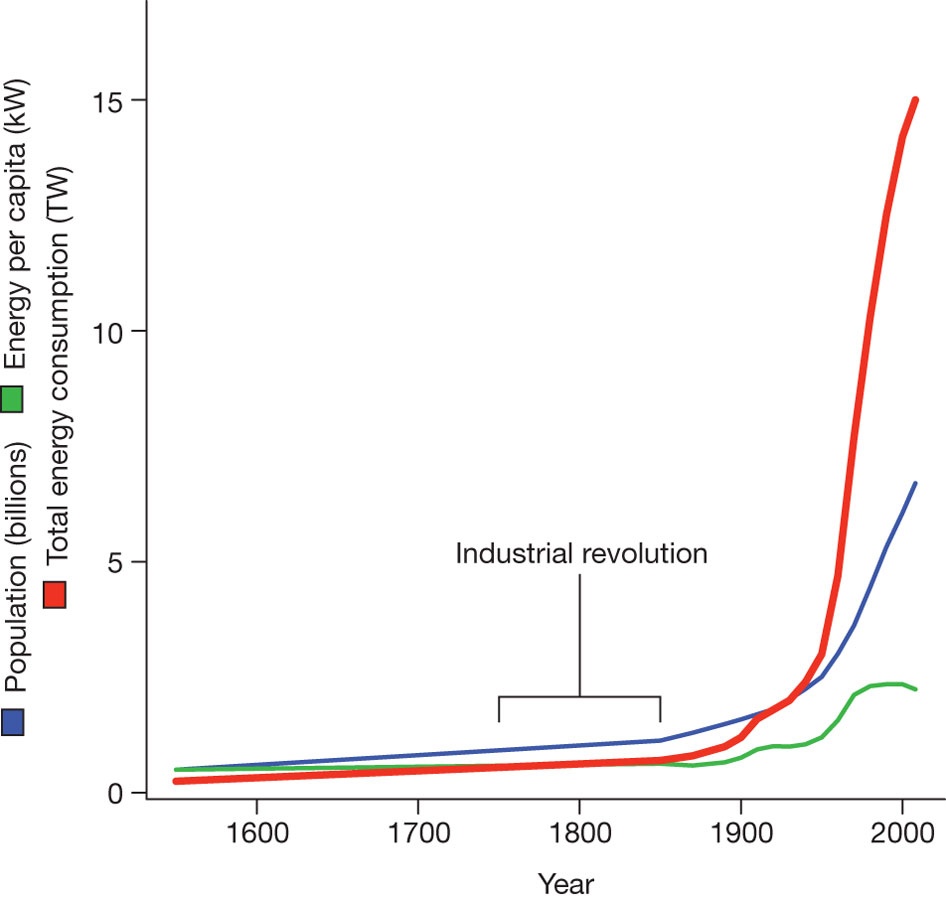
\includegraphics[width=1.00\textwidth]{energy_population.jpg}
	\caption{energy and population, demonstrating the changes -- although we need to be careful to not make assumptions to about causation --- correlation does not necessarily mean causation!}
	\label{fig:energy_population}
\end{figure}



With the initiation of the industrial revolution, we have increasingly relied on high density power. Of these, oil and coal fields are among the most dense (Figure~\ref{}). In terms of the impact on the world, we have...the ``density of power'' demonstrates the value of fossil fuels (Figure~/ref{fig:Power-Densities}), in spite of their areal needs, they remain a compelling source of energy. So, let's talk about fossil fuels and their geologic formations, mining, and processing.

\begin{figure}[h]
	\centering
		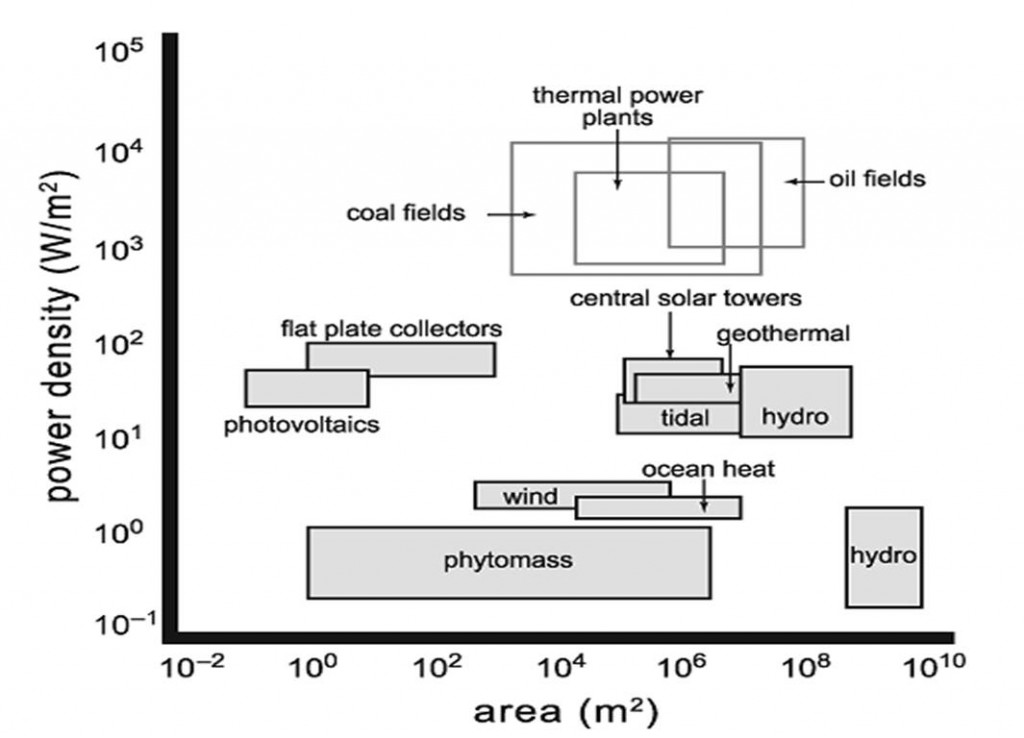
\includegraphics[width=1.00\textwidth]{graphics/Power-Densities.jpg}
	\caption{Characterizing sources of energy based on the area needed versus the density of the power (w2/m2) demonstrates how unique fossil fuels are. }
	\label{fig:Power-Densities}
\end{figure}


\section{Coal, Natural Gas, and Crude Oil}

\subsection{Fossil Fuels and the Environment}

Typically when fossil fuels are studied within the realm of environmental science, we focus on how relying on them for energy contributes to greenhouse gases. In this section, we are going to delve into other ways in which fossil fuels affect the environment. By focusing on the extraction processes of different types of fuels, we will discover the ways in which surrounding ecosystems are directly affected by mining through land subsidence and ground water pollution. We will focus on China, as this is the largest fossil fuel producer and user in all of Asia. 

For example, coal deposits throughout China are burning underground, releasing huge amounts of greenhouse gases, fundamentally changing landscapes, and having serious economic impacts. An estimated 15--20 million tons of coal are burning annually in northern China through these inadvertent fires \citep{kuenzer2007uncontrolled}.

% Citeint ``China: World? Largest Energy Consumer and Greenhouse Gas Emitter"
%   \1 China 2012, coal is 66\% of energy, fossil fuels over 90\%
%   \1 China is estimated to contain over 90 billion tonnes of coal reserves. In 2016, the country produced 2.62 billion tonnes of coal. CITE(world energy council)

%%%%%%%%%%%%%%%%%%%%%%%%%%%%%
%What are fossil fuels
%%%%%%%%%%%%%%%%%%%%%%%%%%%%%

\section{Geologic Processes and Fossil Fuel Production}

\subsection{What are fossil fuels?}

\Gls{fossil fuels} are hydrocarbons, meaning they are composed of hydrogen and carbon. This term typically includes coal, crude oil, and natural gas which all started to form millions of years ago from plant and animal remains. A combination of extremely high temperatures, high pressures, and millions of years allowed these organisms to be transformed into fossil fuels. 

\subsection{Coal Formations}

The first trees evolved around 360 million years ago at the beginning of the Carboniferous period. These ancient trees are the basis for our coal. Coal formation begins with thousands of years of plant accumulation. This process starts with plants in wetland environments dying and beginning to decompose. 
This plant matter is then buried beneath new layers of plants which later die and add to the layers of organic matter beneath them. The resulting partially decomposed plant matter is known as \gls{peat}. In tropical climates, the rate of peat accumulation is estimated to be about 2 meters every century.

Fossil fuel formations are were created in sedimentary basins. For example, the most significant coal formations originated from the detritus of trees, ferns, and other plants that were growing during the Carboniferous ``coal-bearing'' Period 290--360 million years ago. A combination of environmental factors, such as the evolution of large woody trees, allowed for coal deposits to begin to form during this time period. Lesser formations of coal continued through the Permian and Mesozoic Eras, 290--250 and 250--65 million years ago, respectively. Coal deposits that are less than 65 million years in age typically yield low quality coal, as they have not have enough time to fully transform into high-grade coal. 

\begin{figure}[htb]
	\centering
		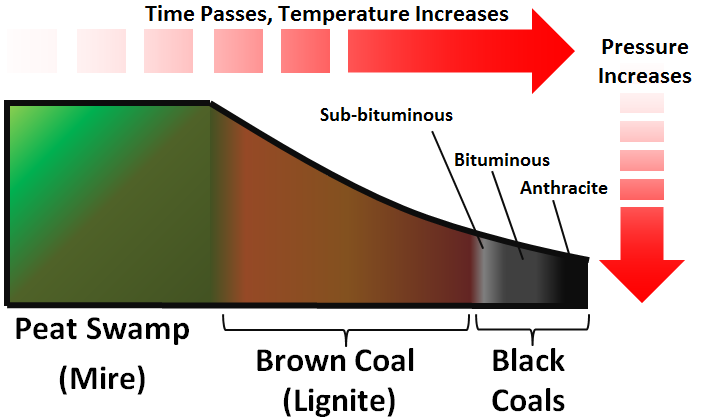
\includegraphics[width=1.00\textwidth]{graphics/CoalFormation.png}
	\caption{Coal formation processes: imagine a nifty graphic probably with a flow-chart vibe, showing the different levels in the coal formation process and the corresponding increasing carbon concentrations}
	\label{fig:CoalFormation}
\end{figure}

As peat transforms to coal (Figure~\ref{fig:CoalFormation}), it is further compacted to be about one-tenth of its original depth. As peat is increasingly buried, the resulting pressure transforms it into \textbf{lignite} which is low quality coal. When comparing the appearance of peat and lignite, we would find peat to contain some undecomposed plant material which lignite lacks. Additionally, lignite forms distinct geological layers \citep{xie2015geological}.

The pressure and temperature continue to increase, allowing the low quality coal to progress to an intermediary sub-bituminous coal and then \textbf{bituminous coal}, the most widely spread type of coal.

Finally, with increasing pressure and a few more million years the high-grade coal, known as \textbf{anthracite}, is formed. The different types of coal contain varying concentrations of carbon: anthracite has the highest concentration which ranges from 86--98\% carbon, while lignite contains about 65--70\% carbon \citep{xie2015geological}.

\subsection{Petroleum and Natural Gas Formation}

In a comparable manner to coal, petroleum and natural gas are formed over long periods of time as organic materials are compressed and heated. We previously saw that coal is formed from decaying terrestrial plants; in contrast, petroleum and natural gas originate primarily from marine plankton.

\begin{figure}[ht]
\centering
    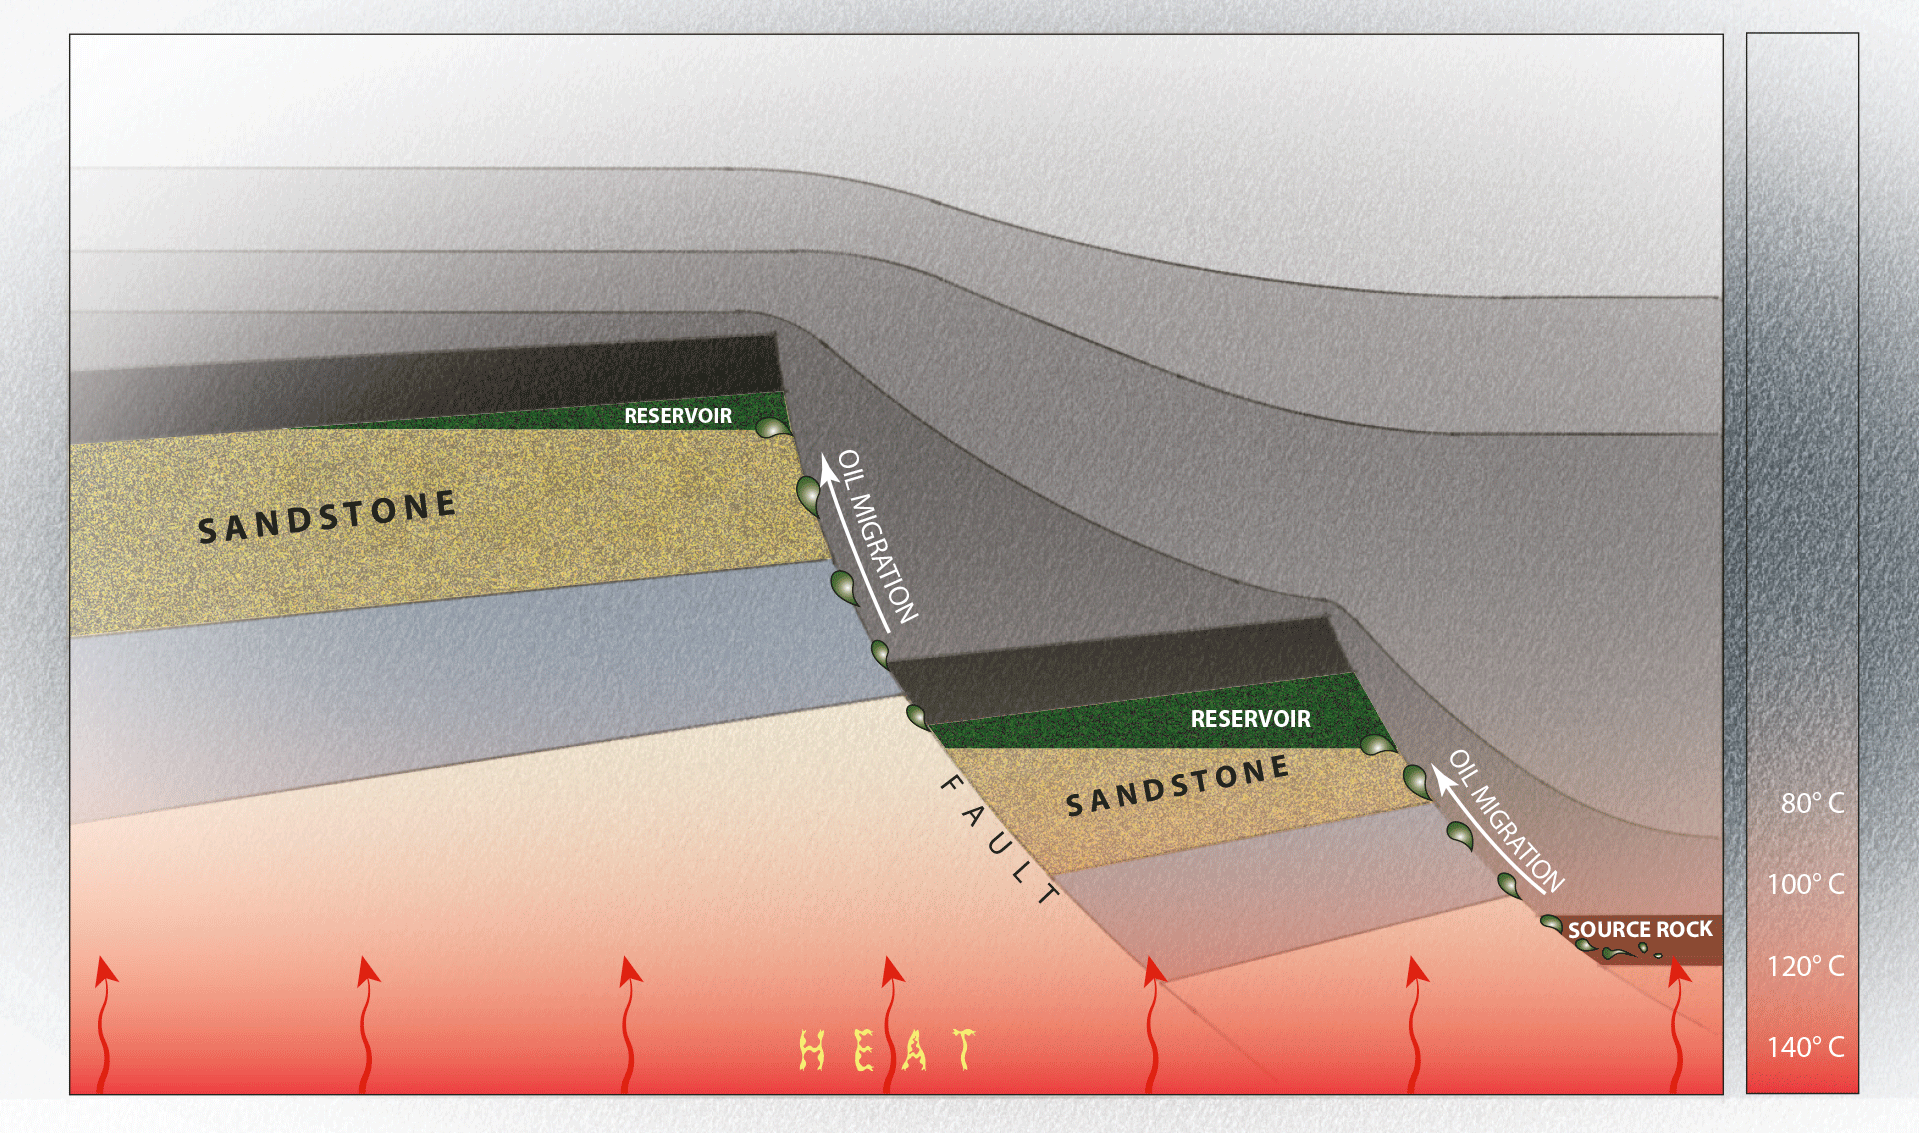
\includegraphics[width = 1\textwidth]{petroform.png}
    \caption{Formation of oil and gas reservoirs. Source: The Norwegian Petroleum Directorate }
    \label{fig:petroform}
\end{figure}

As the phytoplankton died, they sank to the seafloor and accumulated in the oxygen-free environment as sediment deposited on top of them. Similar to the decay process in wetlands, we often speak of diagensis in the marine systems that begin the breakdown process of organic matter on the marine floor.Over time, they became buried over time and like coal were transformed by heat and pressure. 

\section{Extracting Fossil Fuels: Coal Mining}

The first step in coal mining is, of course, is to find the stuff!  Some countries have massive reserves, e.g. the US and China have the most extensive reserves. 

Coal reserves are found throughout China, with recoverable reserves estimated at 324.1 billion tons. Figure~\ref{fig:coallocation} shows where these coal reserves are located throughout the country. The vast majority of this coal is not accessible via surface mining; in fact, only about 5--7 percent can be secured with this method. As of 2010, China was producing coal at a rate of 2.24 billion tons per year, of which surface mining accounted for about 9\%. 

\begin{figure}[ht]
\centering
    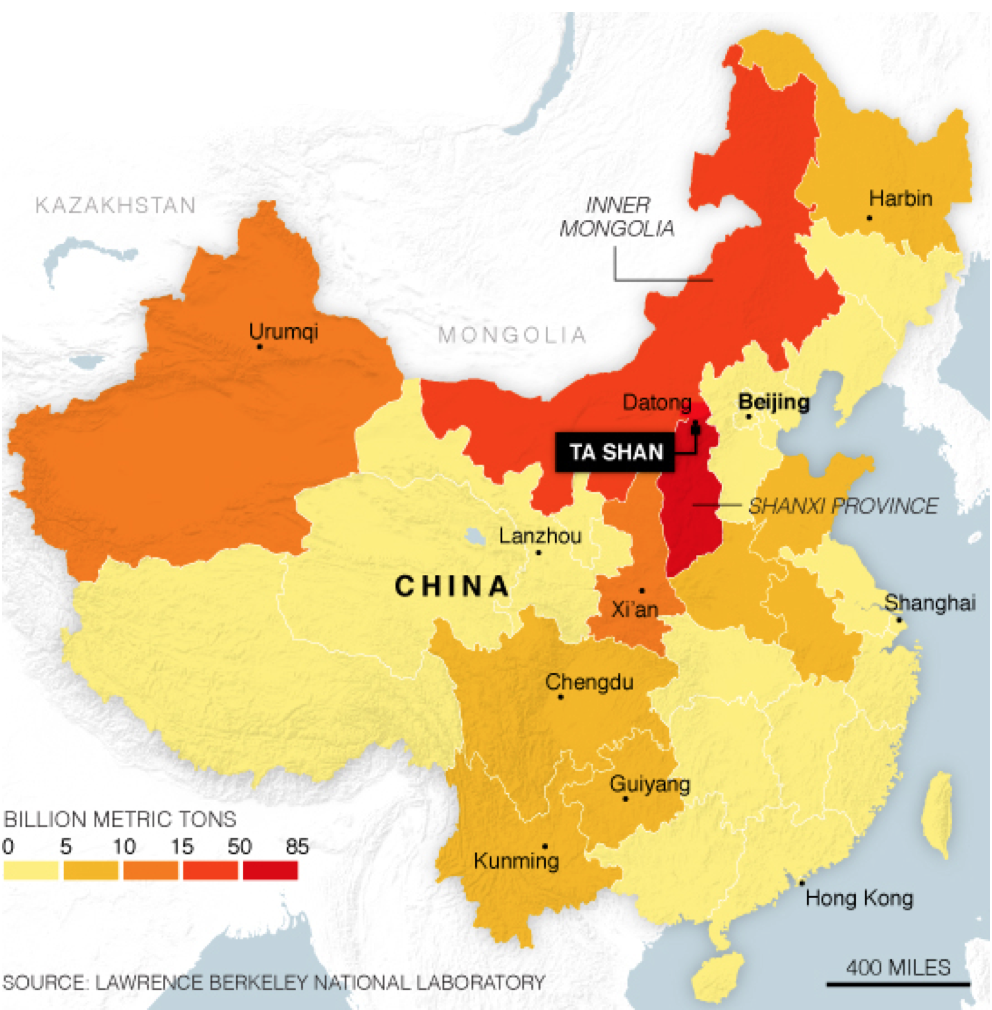
\includegraphics[width = 0.70\textwidth]{coallocation.png}
    \caption{Map of China's technically recoverable coal reserves by province. }
    \label{fig:coallocation}
\end{figure}

\subsubsection{Surface Coal Mining}

There are three distinct surface mining methods that are presently employed in China: open pit mining, area type mining, and contour mining. 

Openpit mining... 


\begin{figure}[ht]
\centering
    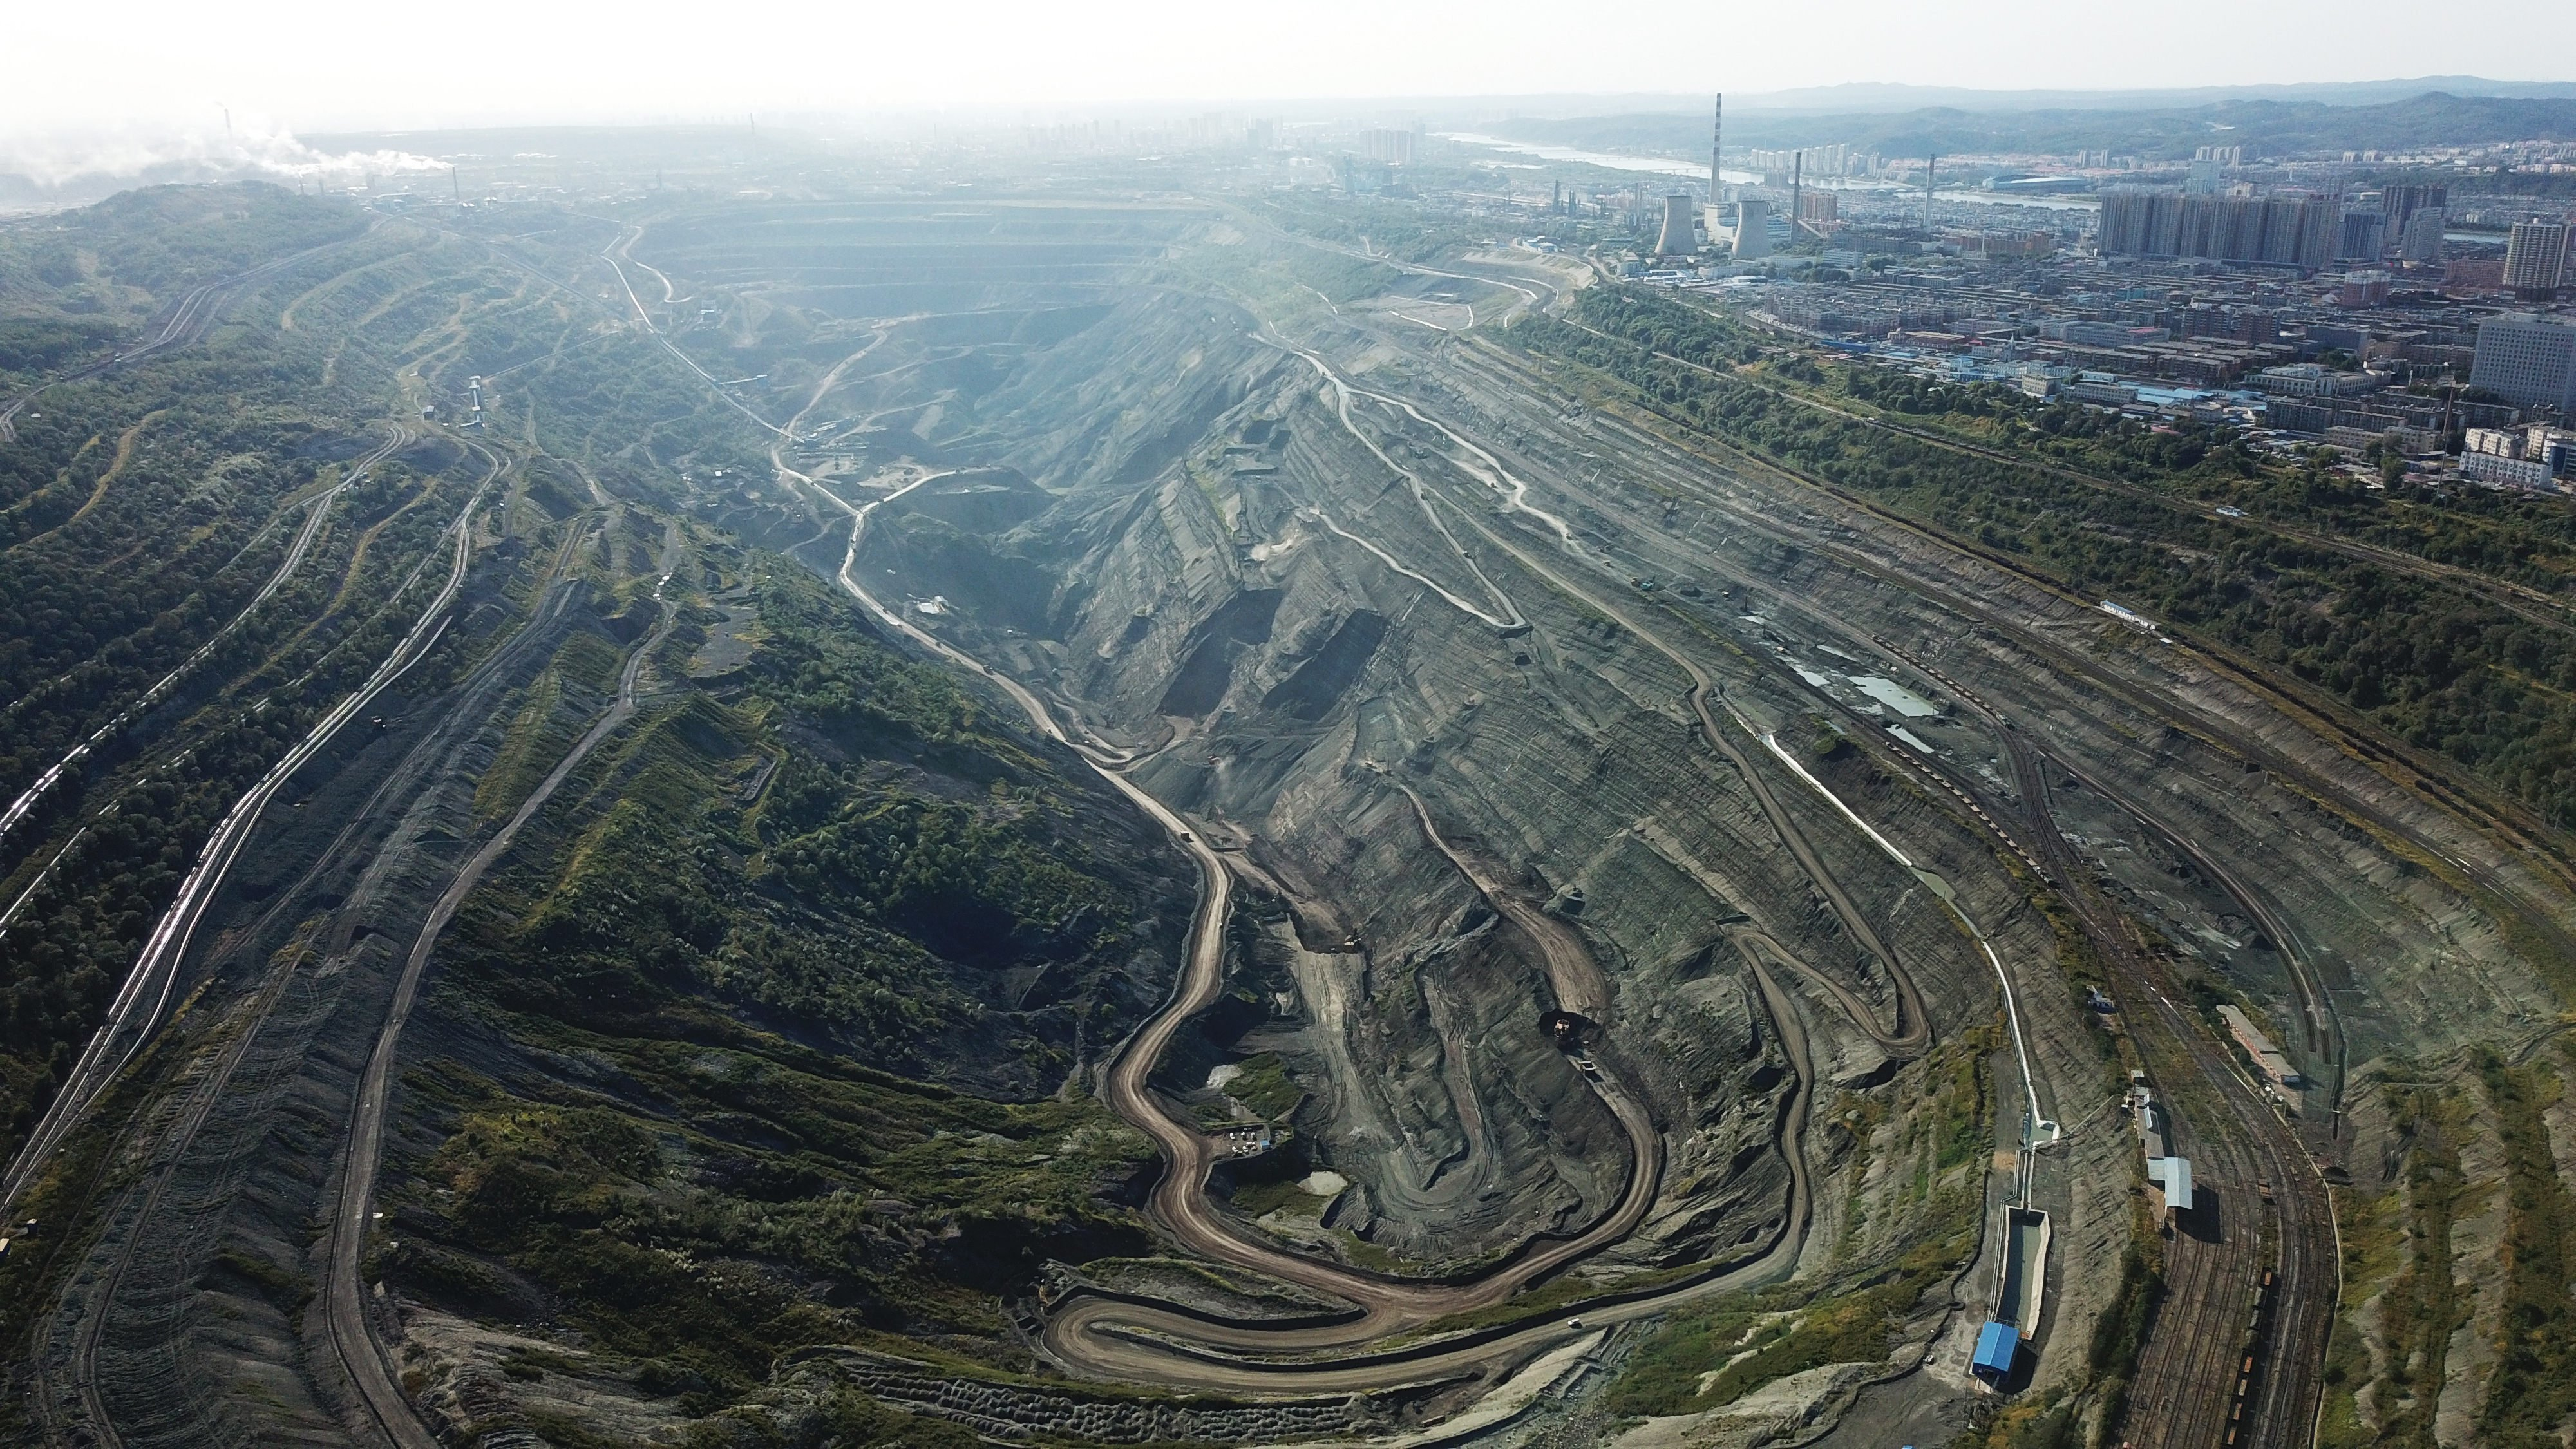
\includegraphics[width = 1.0\textwidth]{openpit.jpg}
    \caption{An open-pit coal mine, located in Fushun, in northeast China's Liaoning province. Source: Image from Yan Bo of Zuma Press. }
    \label{fig:openpit}
\end{figure}

Area type mining is commonly employed in surface coal mines established after 1980 in China. 

In China, area type mining is characterized by the removal of coal seams ranging in thickness from 6 to 30 meters, with some being over 100 meters in thickness. 

Contour mining...



\citep{ji2012surface}


\subsubsection{Underground Coal Mining}


\subsection{Environmental Effects of Coal Mining}

\subsubsection{Fires in China}

Underground coal fires are not a new phenomena. Lightning strikes, grass and forest fires, and spontaneous combustion have all been contributing to coal fires for the past few million years \citep{ceycoal}. It is the frequency of these fires that has significantly increased due to human activity over the past century as more coal deposits are exposed for mining. 

As coal deposits are consumed by fires below ground, \textbf{subsidence} often becomes apparent above ground. Land subsidence refers to the gradual settling or sudden sinking of the Earth's surface. 

%%Cite USGS Groundwater Information: Land Subsidence
The landscape changes in areas surrounding subsurface coal fires are not subtle. Cracks induced by subsidence can measure up to a few meters wide, hundreds of meters deep, and can continue onward for several kilometers in length \citep{stracher2007coal}. %\citep{stracher2004coal}.

These cracks, which often occur on a slightly smaller scale, are part of a positive feedback loop (See Section~\ref{ssub:feedback}). %%%Cite Colin's section about feedback%%%
As coal deposits burn below ground, they create cracks in the ground above them. This gives the fire greater access to oxygen thereby promoting combustion. Consequently the coal continues to burn, causes more subsidence, more burning, and so on. Figure~\ref{fig:undergroundfire} shows how the underground coal fires cause the ground above them to subside and greater air flow increases the fire's capabilities. 


\begin{figure}[ht]
\centering
    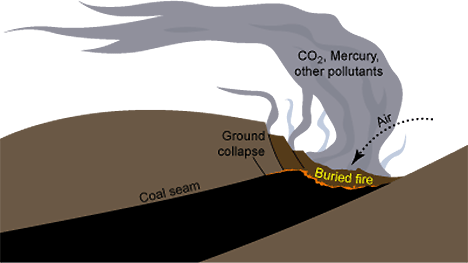
\includegraphics[width = 0.70\textwidth]{undergroundfire.png}
    \caption{Underground coal fire. Schematic showing subsidence and pollution that occurs with underground coal fires (Source: TBD). }
    \label{fig:undergroundfire}
\end{figure}

Coal mining does simply occur in uninhabited areas. The effects of subsidence are apparent in Da Antou, located in Shanxi province about 650 kilometers southwest of Beijing. This small village sits atop a mountain that is littered with underground coal mines. In 2007 the majority of the 200 houses in Da Antou were cracked, and more than a dozen have been declared unfit to be inhabited since 2005. Chen Xiao'e, a former resident of Da Antou, describes how her windows started to shatter before cracks appeared, several centimeters in width, in the walls of her three-year-old brick home. Finally the floor buckled and the house became entirely unsafe to live in. 

\section{Oil and Natural Gas Drilling}

\subsection{Early Oil Drilling [NEEDS REVISING]}

An oil well is a boring in the Earth that is designed to bring petroleum oil hydrocarbons to the surface. Usually some natural gas is released along with the oil. A well that is designed to produce mainly or only gas may be termed a gas well.

The earliest known oil wells were drilled in China in 347 CE. These wells had depths of up to about 240 metres (790 ft) and were drilled using bits attached to bamboo poles.[1] The oil was burned to evaporate brine and produce salt. By the 10th century, extensive bamboo pipelines connected oil wells with salt springs. The ancient records of China and Japan are said to contain many allusions to the use of natural gas for lighting and heating. Petroleum was known as Burning water in Japan in the 7th century.

According to Kasem Ajram, petroleum was distilled by the Persian alchemist Muhammad ibn Zakar?ya R?zi (Rhazes) in the 9th century, producing chemicals such as kerosene in the alembic (al-ambiq), [verification needed] and which was mainly used for kerosene lamps. Arab and Persian chemists also distilled crude oil in order to produce flammable products for military purposes. Through Islamic Spain, distillation became available in Western Europe by the 12th century.

Some sources claim that from the 9th century, oil fields were exploited in the area around modern Baku, Azerbaijan, to produce naphtha for the petroleum industry. These places were described by Marco Polo in the 13th century, who described the output of those oil wells as hundreds of shiploads. When Marco Polo in 1264 visited Baku, on the shores of the Caspian Sea, he saw oil being collected from seeps. He wrote that "on the confines toward Geirgine there is a fountain from which oil springs in great abundance, in as much as a hundred shiploads might be taken from it at one time."[citation needed]

\subsubsection{Modern Drilling}

In 1846, Baku (settlement Bibi-Heybat) the first ever well was drilled with percussion tools to a depth of 21 meters for oil exploration. In 1848, the first modern oil well was drilled on the Absheron Peninsula north-east of Baku, by Russian engineer F.N. Semyenov.

Ignacy ?ukasiewicz, a Polish pharmacist and petroleum industry pioneer built one of the world's first modern oil wells in 1854 in Polish village B\'obrka, Krosno Co who in 1856 built one of the world's first oil refineries.

In North America, the first commercial oil well entered operation in Oil Springs, Ontario in 1858, while the first offshore oil well was drilled in 1896 at the Summerland Oil Field on the California Coast.

The earliest oil wells in modern times were drilled percussively, by repeatedly raising and dropping a cable tool into the earth. In the 20th century, cable tools were largely replaced with rotary drilling, which could drill boreholes to much greater depths and in less time. The record-depth Kola Borehole used non-rotary mud motor drilling to achieve a depth of over 12,000 metres 

\subsubsection{Impacts of Drilling}


\subsection{Predictions of Peak Oil}

The prediction that we might run out of oil has been a re-occurring theme for several generations. Peak oil is the theorized point in time when the maximum rate of extraction of petroleum is reached, after which it is expected to enter terminal decline. Peak oil theory is based on the observed rise, peak, fall, and depletion of aggregate production rate in oil fields over time. It is often confused with oil depletion; however, whereas depletion refers to a period of falling reserves and supply, peak oil refers to peak, before terminal depletion occurs. The concept of peak oil is often credited to geologist M. King Hubbert whose 1956 paper first presented a formal theory.


Peak oil estimates are based on aggregated production of various fields. Oil production forecasts on which predictions of peak oil are based are sometimes made within a range which includes optimistic (higher production) and pessimistic (lower production) scenarios. A 2013 study concluded that peak oil ``appears probable before 2030,'' and that there was a ``significant risk'' that it would occur before 2020, and assumed that major investments in alternatives will occur before a crisis, without requiring major changes in the lifestyle of heavily oil-consuming nations. Pessimistic predictions of future oil production made after 2007 state either that the peak has already occurred, that oil production is on the cusp of the peak, or that it will occur soon.

\begin{figure}[b]
	\centering
		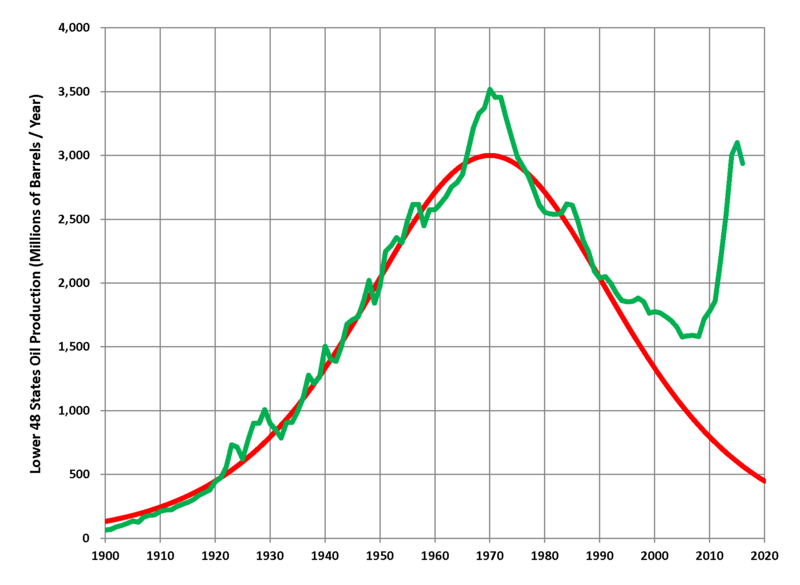
\includegraphics[width=1.00\textwidth]{graphics/Hubbert_Upper-Bound_Peak_1956.png}
	\caption{peak oil}
	\label{fig:Hubbert_Upper-Bound_Peak_1956}
\end{figure}

Hubbert's original prediction that US peak oil would occur in about 1970 appeared accurate for a time, as US average annual production peaked in 1970 at 9.6 million barrels per day and mostly declined for more than 3 decades after. However, the use of hydraulic fracturing caused US production to rebound during the 2000s, challenging the inevitability of post-peak decline for the US oil production (Figure~\ref{fig:Hubbert_Upper-Bound_Peak_1956}). Thus, we need to address recent changes in the technology to extract oil reserves.

\subsection{Hydraulic fracturing (fracking)} 

Hydraulic fracturing, known more commonly as \textbf{fracking}, is an extraction method used to remove gas and oil from within impermeable shale rock. But the technology relies on several other changes to oil exploration and drilling. 

Until the 1970s, most oil wells were vertical, although lithological and mechanical imperfections cause most wells to deviate at least slightly from true vertical. However, modern directional drilling technologies allow for strongly deviated wells which can, given sufficient depth and with the proper tools, actually become horizontal. This is of great value as the reservoir rocks which contain hydrocarbons are usually horizontal or nearly horizontal; a horizontal wellbore placed in a production zone has more surface area in the production zone than a vertical well, resulting in a higher production rate. The use of deviated and horizontal drilling has also made it possible to reach reservoirs several kilometers or miles away from the drilling location (extended reach drilling), allowing for the production of hydrocarbons located below locations that are either difficult to place a drilling rig on, environmentally sensitive, or populated.

Hydraulic fracturing requires vertically drilling downward for about 2 km before turning to drill horizontally for as far as 3 km.  The fracking process itself is based in expelling fracking fluid, known as \textbf{slickwater}, at high pressures through small perforations in the horizontal pipe. The slickwater, composed of water, sand, and an assortment of additives, is forced out of the horizontal pipe at pressures above 600 atm creating microfractures for up to 50 m in the surrounding rock.

Thus, Hubbert's original predictions for world peak oil production proved premature. Nevertheless, the rate of discovery of new petroleum deposits peaked worldwide during the 1960s and has never approached these levels since.

\subsection{Environmental Concerns with Oil Drilling}

There are a number of environmental concerns surrounding fracking. 


\begin{itemize}
\item Water usage 

The fracking process requires extremely large volumes of water. INSERT NUMBER. Sourcing this much water can put a stress on surrounding surface and ground water reserves, particularly in desert regions such as INSERT LOCATION.

\item Water contamination 

The flowback liquid from fracking contains the original additives and may also contain heavy metals, radioactive material, and other toxins. Poorly constructed wells or other means of spilling this liquid could contaminate surrounding surface and ground water sources. 



\item Subsidence

As with other forms of fossil fuel extraction, removing and altering material from below ground tends to cause subsidence.

\item Methane

\begin{figure}[h]
	\centering
		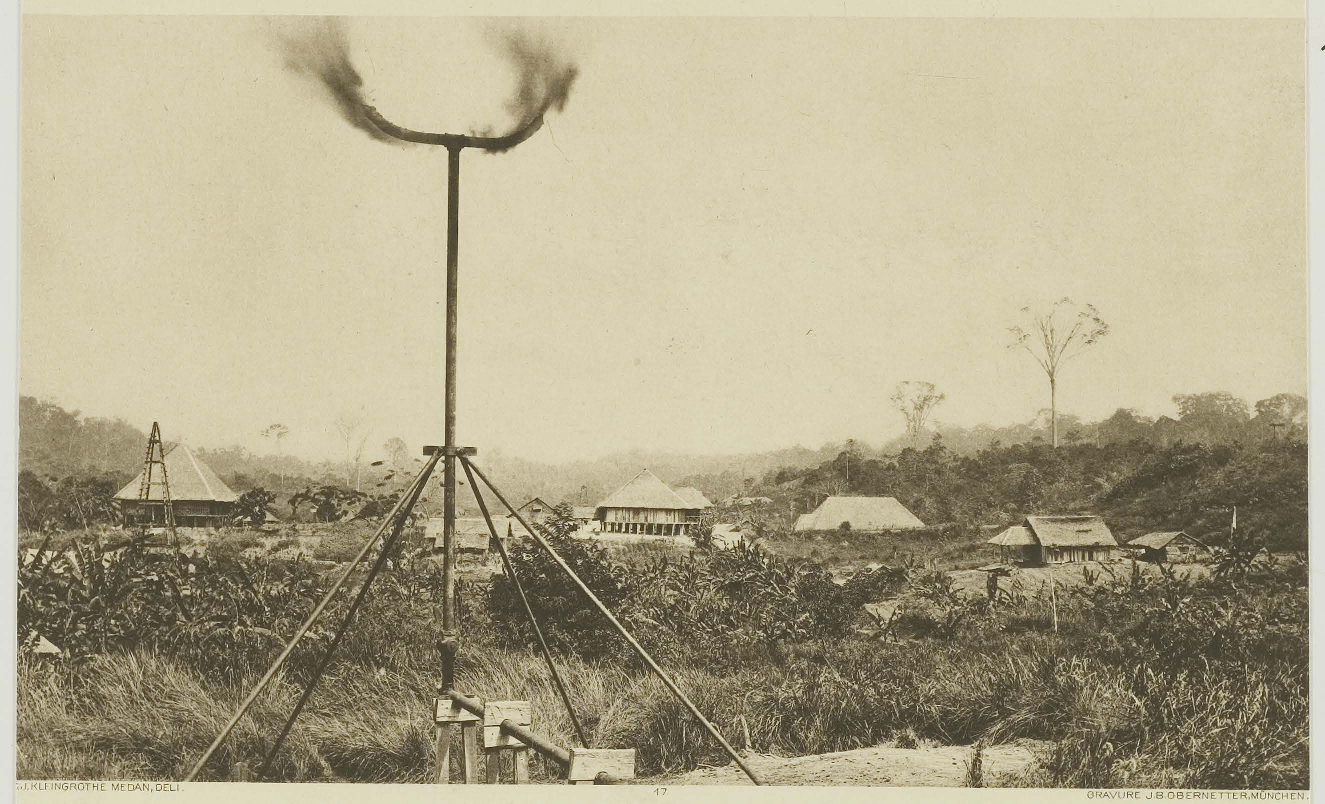
\includegraphics[width=1.00\textwidth]{graphics/Burning_of_natural_gases_Sumatra}
	\caption{Burning of natural gases at an oil drilling site, presumably at Pangkalan Brandan, East Coast of Sumatra - circa 1905}
	\label{fig:Burning_of_natural_gases_Pangkalan_Brandan_Sumatra}
\end{figure}


\end{itemize}


\section{A Fossil Fuel Addiction}

\subsection{Supply and Demand}

\emph{The goal of this section is to show that while there are serious environmental/health effects associated with fossil fuels, we can't simply stop using them. I'll show that China, while incredibly dependent on coal, is actually one of the most efficient countries at processing coal. }

Let's now take a step back and briefly examine the economic and political reasons why countries like China are so dependent on fossil fuels and in particular, coal.  



\subsection{Fossil Fuels and Asia}

While China is incredibly dependent on coal, its coal-fired power plants are significantly more efficient that those in the United States. In this context, efficiency refers to the amount of coal consumed per unit of power produced, and is thus related to gas emissions. 

Rapid growth, etc, etc, etc, relatively cheap option, reserves, etc

\subsection{Development and Greenhouse Gas Emissions}

\subsection{Does Development Depend on Burning Fossil Fuels?}

Some observers, such as petroleum industry experts Kenneth S. Deffeyes and Matthew Simmons, predicted there would be negative global economy effects after a post-peak production decline and subsequent oil price increase because of the continued dependence of most modern industrial transport, agricultural, and industrial systems on the low cost and high availability of oil. Predictions vary greatly as to what exactly these negative effects would be. While the notion that petroleum production must peak at some point is not controversial, the assertion that this must coincide with a serious economic decline, or even that the decline in production will necessarily be caused by an exhaustion of available reserves, is not universally accepted.

%%%%%%%%%%%%%%%%%%%%%%%%%%%%%
%The Economics, my main focus
%%%%%%%%%%%%%%%%%%%%%%%%%%%%%

% \section{Underground Coal Fires in China} \cite{stracher2004coal}
%   \1 Cracks induced by subsidence measuring up to ``several kilometers long, tens of meters wide, and hundred of meters deep"
%       \2 Positive feedback loop- cracks increase oxygen circulation thereby promoting combustion 
%   \1 Economic loss estimated to be as high as \$25-250 million USD (Prakarsh)




